\chapter{Conceitos Básicos}
\label{ch:2}
Neste capítulo discutiremos alguns conceitos básicos necessários ao entendimento da solução proposta. Abordaremos inicialmente orientação a serviços e componentes, apresentando as principais características de cada abordagem. Apresentaremos também a plataforma OSGi e o Framework iPOJO, que são as tecnologias que formam o núcleo deste trabalho. Em seguida, discutiremos sobre gerenciamento de recursos e serviços, sua importância no contexto de arquiteturas orientadas a serviços, e uma visão geral do ciclo de desenvolvimento PDCA, que é um acrônimo das etapdas do ciclo (\textit{Plan}, \textit{Do}, \textit{Check}, \textit{Act}). Por fim, apresentaremos uma visão geral de JMX, a tecnologia utilizada no trabalho para realizar o monitoramento dos recursos.

\section{Orientação a Serviços}
\label{sec:service}

Orientação a Serviços é um paradigma de desenvolvimento de aplicações distribuídas que utiliza serviços como unidades que representam funcionalidades da aplicação atendendo as necessidades do negócio~\cite{erl2008soa}~\cite{cervantes2005technical}. 

Desta forma, serviços descrevem suas capacidades através de interfaces bem definidas e utilizam-se de uma descrição de serviço (\textit{Service Description}) para expor tais capacidades e eventuais propriedades específicas, por exemplo, propriedades relacionadas a requisitos de qualidade ou localização do serviço. Um exemplo conhecido de uma \textit{service description} é o documento WSDL, utilizado para descrever \textit{Web Services} expondo, além da interface do serviço, um conjunto extra de propriedades.

Deste modo, no mundo de serviços, temos diversas implementações distintas para um mesmo serviço, onde o consumidor pode não estar vinculado a nenhuma delas, podendo substituir o serviço consumido de acordo com suas necessidades, através da definição de novos contratos de serviço com base nessas descrições~\cite{cervantes2005technical}.

\subsection{\textit{Service Oriented Architecture}}
Alinhado a essas idéias, temos em SOA, um modelo de arquitetura baseada em serviços com suporte à descoberta dinâmica de serviços. O modelo arquitetural de SOA baseia-se nos 3 elementos fundamentais da orientação a serviços.

\begin{itemize}
 \item \textbf{Provedor de Serviços} (\textit{Service Provider})
 \item \textbf{Consumidor de Serviços} (\textit{Service Requestor})
 \item \textbf{Registro de Serviços} (\textit{Service Registry})
\end{itemize}

A interação destes elementos compõe o tradicional triângulo SOA, ver Figura \ref{fig:soatriangle}. A interação dos elementos é relativamente simples. Provedores de serviço publicam suas capacidades através de \textit{Service Descriptions} no registro de serviços. O consumidor do serviço executa consultas a um determinado serviço, com base em sua descrição, através do registro. Caso exista um provedor que atenda as necessidades do consumidor, então o registro devolverá uma referência do provedor do serviço ao consumidor, possibilitando a realização do \textit{binding} entre eles. Então, o provedor disponibiliza um objeto que implementa a interface do serviço e representa o objeto remoto, em tempo de execução (\textit{Servant}~\cite{volter2005remoting}), finalizando a interação com o provedor. 

Quando a interação entre o consumidor e o \textit{servant} é finalizada, o mesmo é liberado para utilização em alguma outra requisição ou simplesmente destruído. Nesse contexto, o consumidor não tem conhecimento de como o serviço é implementado, onde o mesmo se localiza, nem mesmo se o \textit{servant}, pelo qual ele tem acesso ao serviço, é o mesmo a cada invocação. Esse grau de transparência provê um grande potencial de dinamismo e reuso, que são duas das principais características de arquiteturas orientadas a serviços~\cite{davis2009open}.


\section{Orientação a Componentes}
\label{sec:component}
Segundo Szyperski ~\cite{szyperski2002component}, "Componentes de software são unidades binárias de produção, aquisição e implantação independente, que interagem formando sistemas". Componentes possuem interfaces e dependências através de um modelo de componente. Esses modelos, assim como classes da orientação a objetos, descrevem as características do componente (ver \ref{sub:elements}).

A orientação a componentes também define o conceito de \textit{containers}, que gerenciam o ciclo de vida e encapsulam os componentes, intermediando sua interação com o mundo externo.

Um componente possui 3 propriedades características:

\begin{enumerate}
\item \textbf{Pode ser implantado de forma independente}: Diz respeito a implantação independente de ambiente ou de outros componentes;

\item \textbf{Não deve possui estado observável}: Diz respeito as instâncias de componentes, que não devem ser distinguíveis entre si, ou seja, não há o conceito de estado observável presente na orientação a objetos. Terceiros não conseguem diferenciar cópias de um componente; e

\item \textbf{Unidade de composição com terceiros} Essa propriedade traz consigo algumas características semelhantes as da orientação a serviços, uma vez que, para a realização de uma composição, o componente deve ser coeso, auto-contido e possuir interfaces bem definidas. Um componente pode ser visto como uma caixa preta, que encapsula detalhes de sua implementação e interage com o mundo externo através de sua(s) interface(s).
\end{enumerate}

Essas propriedades são realizadas por 3 elementos distintos que são base da orientação a componentes.

\subsection{\textit{Component Elements}}
\label{sub:elements}

\subsubsection{Modelo de Componente}
O conceito de modelo de componente é, de certa forma, similar ao conceito de classe na orientação a objetos~\cite{cervantes2005technical}. Ele abstrai e descreve as características dos componentes (interfaces, propriedades, dependências) e pode definir mecanismos pelos quais estes são implantados.

\subsubsection{Instância de Componente}
Uma instância de componente, retomando nossa analogia a orientação a objetos, é um elemento que representa uma entidade "física" do modelo. Diferente do modelo, uma instância de componente possui estado e pode fazer parte de composições~\cite{cervantes2005technical}~\cite{szyperski2002component}.

\subsubsection{Pacote de Componente}
Um pacote de componente pode ser definido como um componente pronto para ser implantado, ou seja, um componente auto-contido que possui todas as suas dependências resolvidas de maneira a prover suas funcionalidades de forma independente~\cite{cervantes2005technical}.

\subsection{\textit{Deployment Descriptors}}
Outro elemento importante no mundo de componentes é o chamado \textit{Deployment Descriptor}, que é um arquivo de configuração que descreve um conjunto de propriedades que definem como o componente será implantado na plataforma~\cite{deploy}~\cite{deployoasis}. 

Geralmente essas propriedades são descritas em documentos XML~\cite{xml} devido a sua natureza semi-estruturada, representatividade e a facilidade de entendimento e escrita. 
\section{OSGi}
\label{sec:osgi}

Como é amplamente conhecido, Java fornece a portabilidade necessária para suportar aplicativos em diferentes plataformas, porém, não dá suporte explícito à construção de sistemas modulares~\cite{hall2010osgi}. A plataforma OSGi provê um conjunto de especificações permitindo que aplicações sejam construídas de maneira colaborativa, a partir de pequenos componentes reutilizáveis ~\cite{osgiorg}, simplificando o desenvolvimento e a manutenção do código~\cite{hall2010osgi}.

O principal componente da especificação OSGi é o Framework OSGi, ele fornece um ambiente padronizado onde as aplicações, denominadas \textit{bundles}, podem, em tempo de execução,  ser instaladas, desinstaladas, ativadas ou desativadas local ou remotamente.


\subsection{Arquitetura}

A arquitetura do OSGi define um conjunto de camadas, vistas na Figura \ref{fig:arch_osgi}. 

Iremos nos concentrar nas principais camadas do framework, apresentando-as nas próximas sub-seções.

\begin{figure}[htp]
\centering
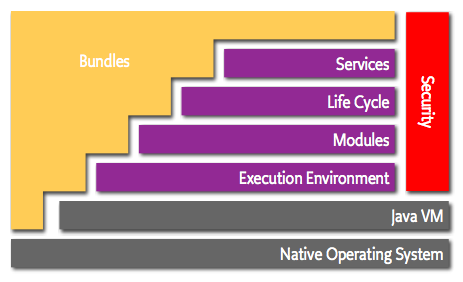
\includegraphics[width=9cm]{chapters/chapter2/arch-osgi.png}
\caption[Arquitetura OSGi]{Arquitetura OSGi~\cite{osgiorg}.}
\label{fig:arch_osgi}
\end{figure}


\subsubsection{\textit{Module Layer}}
Define o conceitos de módulos, providos através dos \textit{Bundles}. Um \textit{bundle} é um arquivo JAR com um conjunto de metadados definidos em um \textit{Manifest}. De fato, a figura do \textit{bundle} é extremamente simples, porém, ao mesmo tempo poderosa, uma vez que, diferente de um simples arquivo JAR, um \textit{bundle} define um módulo lógico que pode ser combinado para a composição de uma aplicação~\cite{hall2010osgi}.

Além disso, ~\textit{bundles} podem declarar explicitamente dependências externas e pacotes exportados, ampliando o mecanismo de controle de acesso padrão de Java. Essa capacidades de declarar explicitamente pacotes importados e exportados, traz um grande benefício ao desenvolvedor, uma vez que, o próprio framework fica responsável por gerenciar e verificar automaticamente a consistência da aplicação, através de um processo chamado \textit{bundle resolution}~\cite{hall2010osgi}~\cite{osgiorg}.

\subsubsection{\textit{Lifecycle Layer}}
A camada de ciclo de vida controla o ciclo de vida dos \textit{bundles}, definindo como os mesmos são gerenciados (instalados, desinstalados,parados, etc.) dinamicamente em tempo de execução.

Ela também define como os \textit{bundles} obtém acesso ao \textit{bundle context}, além de ser responsável por controlar a interação dos \textit{bundles} com o framework.

Nesse contexto temos a figura do ativador do \textit{bundle}, que se reposabiliza pela inicialização/parada o \textit{bundle}. Provido através da interface \textit{BundleActivator}, que realiza uma função semelhante ao \textit{main} de um programa Java.

\subsubsection{\textit{Service Layer}}
A camada de serviços incorpora características de SOA no OSGi, com as figuras do registro, provedor e consumidor de serviço, visto na Seção \ref{sec:service}. Ela expande o dinamismo provido pelos \textit{bundles} na camada de ciclo de vida, combinando-o ao dinamismo provido por arquiteturas orientadas a serviço, onde serviços podem aparecer ou desaparecer a qualquer momento~\cite{hall2010osgi}.

\subsection{iPOJO}
\label{subsec:ipojo}
Outra tecnologia importante para a compreensão deste trabalho, é o framework iPOJO~\cite{ipojo}. O iPOJO implementa um modelo componentes orientados a serviço, e tem como principal objetivo simplificar o desenvolvimento de aplicações OSGi. O iPOJO utiliza o conceito de POJO (\textit{Plain Old Java Objects}) para definir componentes, onde um POJO é basicamente um objeto java simples, que não possui nenhuma dependência do ambiente de execução.
	
No iPOJO, os diversos POJO's são encapsulados em \textit{containers}, responsáveis pelo gerenciamento das interações entre o POJO e o mundo externo ao \textit{container} e podem ser estendidos através da utilização de \textit{handlers}~\cite{ipojo}.

\begin{figure}[htp]
\centering
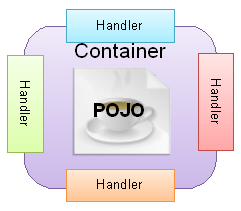
\includegraphics[width=5cm]{chapters/chapter2/ipojo-handlers.png}
\caption[Handlers Ipojo]{Handlers iPOJO~\cite{ipojo}.}
\label{fig:arch_osgi}
\end{figure}

O iPOJO se baseia nos conceitos de orientação a componentes, onde temos, além da figura do \textit{container}, a visão de modelo e instância de componente. No iPOJO, o modelo de componente, chamado de \textit{component type}, especifica: um conjunto de propriedades do componente, sua classe de implementação e políticas de criação de instâncias. Cada instância do componente herda todas as características do \textit{component type} e pode ter seu próprio conjunto de propriedade~\cite{ipojo}.

O iPOJO abstrai o uso de OSGi através do conceito de \textit{containers} que controlam o acesso e gerenciam o ciclo de vida do POJO, e de \textit{handlers} ``plugados'' aos \textit{containers} estendendo suas capacidades.


\section{JMX}
\textit{Java Management Extensions} (JMX) é uma API que fornece uma maneira simples e padrão de gestão e monitoramento de recursos para a plataforma Java. Estes recursos podem ser aplicações, dispositivos, serviços ou a própria JVM (\textit{Java Virtual Machine}) e são instrumentados por um ou mais \textit{Managed Beans}, ou simplesmente MBeans, responsáveis por adquirir, manipular ou enviar informações acerca destes recursos~\cite{lindfors2002jmx}.

A especificação de JMX define, além da arquitetura, padrões de projeto, API's e um conjunto de serviços de gerenciamento e monitoramento, que possibilitam o desenvolvimento de aplicações gerenciáveis local ou remotamente através do processo de instrumentação, onde atributos, configurações e capacidades da aplicação são expostos. Isso aumenta a robustez e extensibilidade da aplicação, uma vez que, é possível construir soluções de gerenciamento inteligentes, interoperáveis e independentes da infra-estrutura de gestão~\cite{jmx}.

\subsection{Arquitetura}
\label{subsec:arch}
A arquitetura JMX é definida em três níveis, ver Figura \ref{fig:arch_jmx}:

\begin{itemize}
 \item Nível de Instrumentação;
 \item Nível de Agente;
 \item Nível de Gerenciamento.
\end{itemize}

JMX foi definida segundo duas JSRs , JSR 3 e JSR 160. Os dois primeiros níveis da arquitetura (Instrumentação e Agente) foram definidos na JSR 3, enquanto o Nível de Gerenciamento foi definido na JSR 160. Isso mostra, de certa forma, o potencial de extensibilidade da tecnologia.

\begin{figure}[htp]
\centering
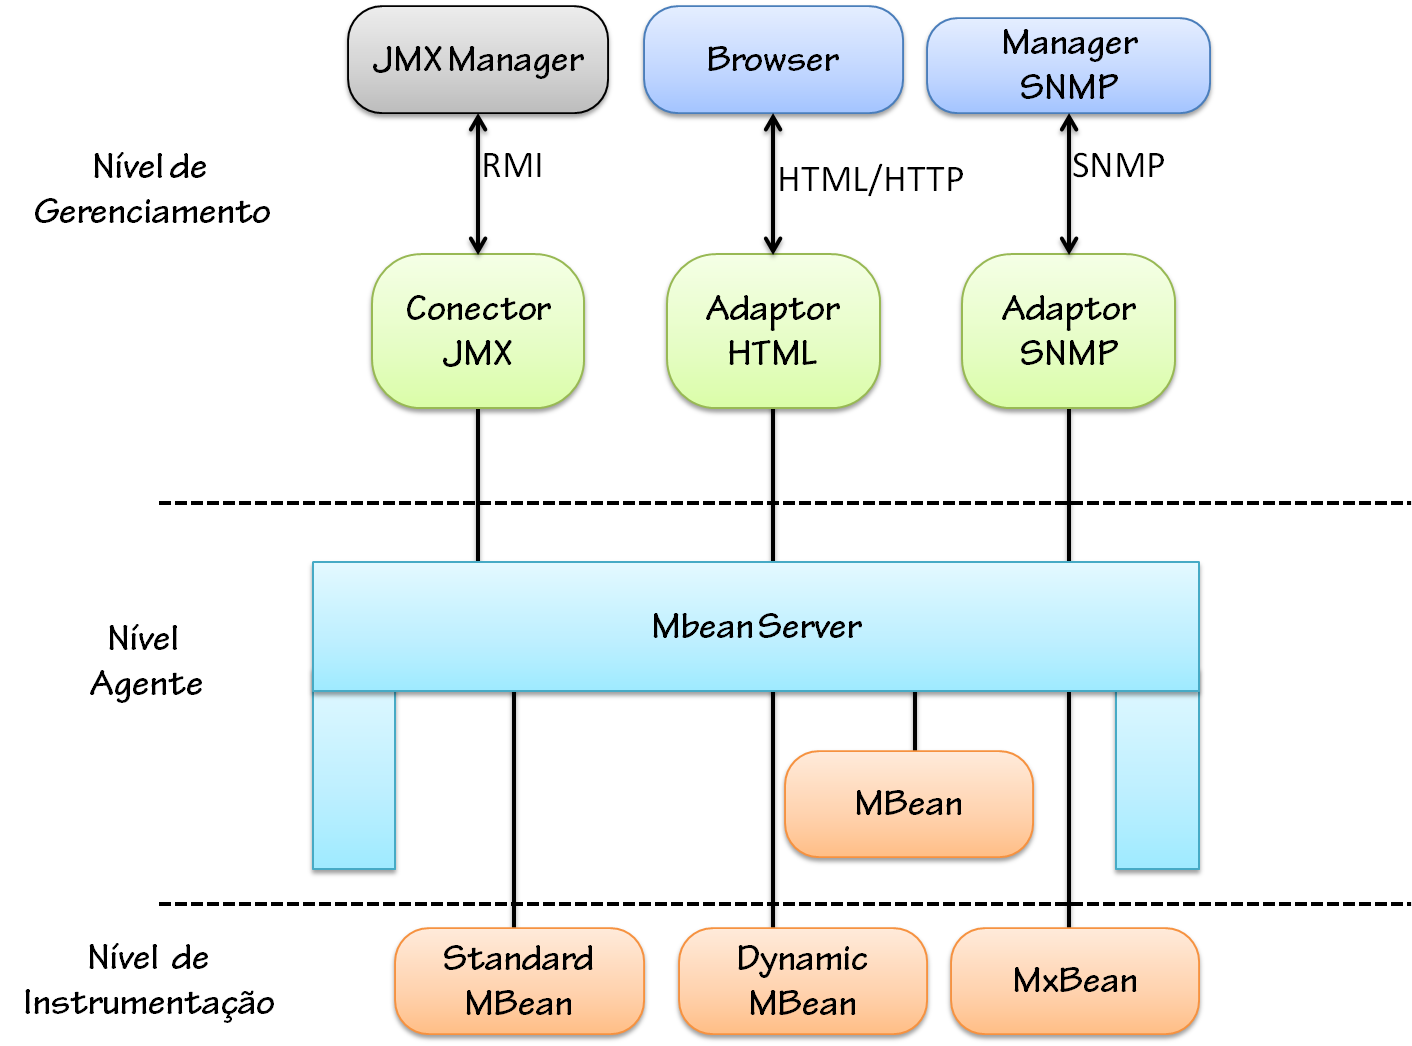
\includegraphics[width=12cm]{chapters/chapter2/arch_jmx.png}
\caption[Arquitetura JMX]{Arquitetura JMX.}
\label{fig:arch_jmx}
\end{figure}

\subsubsection{Nível de Instrumentação}
O nível de instrumentação é responsável por expor as funcionalidades e configurações das aplicações através da criação e registro de MBeans~\cite{jmx}. Estes MBeans coletam e manipulam informações dos recursos gerenciáveis, repassando-as aos agentes JMX do nível superior.

Existem diferentes tipos de MBeans em JMX. Nas próximas sub-seções descreveremos alguns dos mais importantes.

\paragraph{Standard MBean:}
\label{para:stardardmbean}
São os tipos mais simples de \textit{Managed Bean}. Eles interagem com os recursos gerenciáveis através da definição de uma interface de gerenciamento, que descreve os atributos e operações do MBean. Estas interfaces são definidas explicitamente e os atributos e métodos descobertos por meio de reflexão. Além disso, \textit{Standard MBeans} seguem a convenção do nome da classe acrescido do prefixo \verb MBean  e todos os seus atributos são acessados por métodos \textit{getters} e \textit{setters}. \textit{Standard Mbeans} possuem uma limitação quanto aos tipos de dados que podem ser utilizados, não permitindo o uso de tipos complexos definidos pelo usuário~\cite{mxbeans}.

Uma limitação da arquitetura JMX é que não é permitido a implementação de duas interfaces de gerenciamento para o mesmo MBean, mesmo através de herança. Isto evita a implementação explícita de duas interfaces, pois o agente JMX sempre irá utilizar a interface de gerenciamento mais próxima da classe, ou seja, a interface implementada pela própria classe e não pela classe ancestral. Uma alternativa a esse problema é estender a interface de gerenciamento.

\paragraph{MxBean:}
\label{para:mxbean}
Mxbean é uma versão melhorada do \textit{Standard MBean} que possui uma solução ao problema relacionado ao conjunto limitads de tipos de dados utilizáveis pelo MBean comum. Ele provê suporte à utilização de tipos de dados complexos para representação de atributos do MBean, através de mapeamentos de tipos complexos para um tipo padrão \verb CompositeDataSupport ~\cite{mxbeans}.

\paragraph{Dynamic MBean:}
\label{para:dynamicmbean}
\textit{Dynamic MBeans} se diferenciam do \textit{Standard MBeans} pelo fato de que aqueles descrevem seus atributos e operações através de uma interface genérica. Assim, as propriedades do MBean são descobertas em tempo de execução, já que, através dessa interface, os agentes JMX obtém a descrição do MBean por meio da classe \verb MBeanInfo ~\cite{jmx}. Na prática, o diferencial é que no caso dos \textit{Standard MBeans}, os metadados que descrevem a interface são obtidos por meio de reflexão, e no \textit{Dynamic MBean}, as classes de metadados são construídos por elas mesmas em tempo de execução. Desde modo, o acesso ao atributos e operações em MBeans dinâmicas não é realizado diretamente, mas sim por meio de métodos genéricos, semelhante ao mecanismo utilizado pelo padrão de projeto \textit{Requestor}~\cite{volter2005remoting}. Esse método de acesso é ilustrado na figura \ref{fig:requestjmx}.

\begin{figure}[htp]
\centering
\subfloat[Invocação de Operação no MBean]{
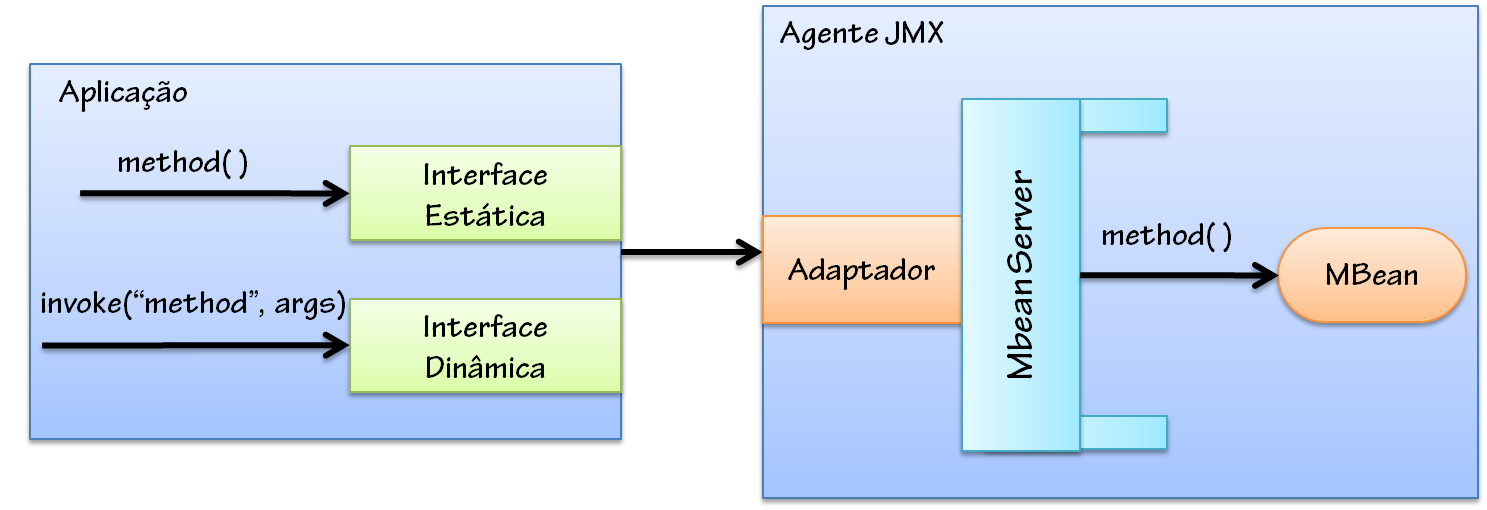
\includegraphics[width=13cm]{chapters/chapter2/invoke.png}
}
\\
\subfloat[Acesso a atributo no MBean]{
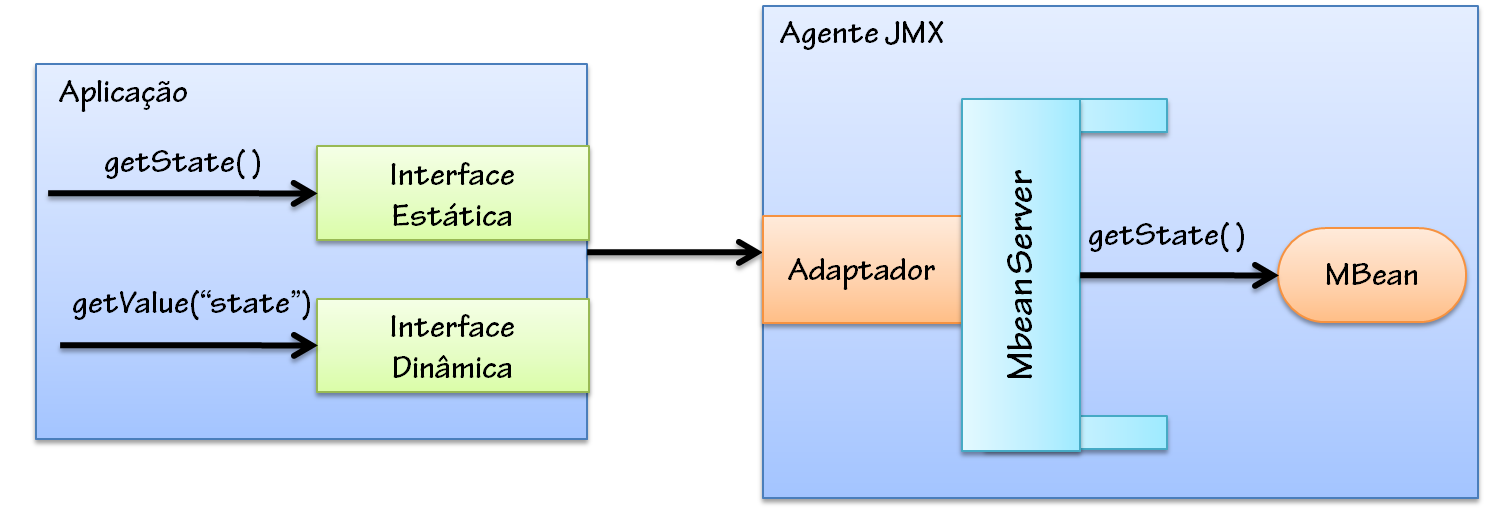
\includegraphics[width=13cm]{chapters/chapter2/getValue.png}
}
\caption{Acesso a atributos e operações do MBean.}
\label{fig:requestjmx}
\end{figure}

Exitem outros tipos de MBeans dinâmioas, como \textit{Model MBean}, \textit{Open MBean} e \textit{AbtractDynamicMBean} que basicamente adicionam novas \textit{features} ao \textit{Dynamic MBean} tradicional. 

\subsubsection{Nível Agente}
O nível agente é responsável por gerenciar todos os \textit{Mbeans} e através delas controlar diretamente todos os recursos, tornando-os acessíveis a aplicativos de gerenciamento remoto.

A gerência dos \textit{MBeans} é provida através do principal componente do agente JMX, o \textit{MBean Server}. Além disso, agentes JMX incluem um conjunto de serviços de gerenciamento de \textit{MBeans} e pelo menos um adaptador de comunicações ou conector para permitir o acesso ao agente por aplicativos de gerenciamento~\cite{jmx}. Basicamente, um agente JMX consiste em um \textit{MBean Server}, um conjunto de serviços básicos de gerência e pelo menos um adaptador de comunicação ou conector JMX.

\paragraph{MBean Server:}
O \textit{MBean Server} é o principal componente do nível agente. Ele é o intermediário entre o sistema de gerenciamento e os objetos gerenciáveis (recursos), uma vez que, é responsabilidade do \textit{MBean Server} registrar e manipular os \textit{MBeans}~\cite{jmx}.

Para registrar um \textit{MBean} no servidor, além do próprio objeto \textit{MBean}, é necessário que seja registrado junto ao \textit{MBean} um \textit{ObjectName} que identifica unicamente aquele \textit{MBean} no servidor. Além de identificar o \textit{MBean}, ele permite a seleção de objetos a partir de máscaras no formato [domínio]:[par chave/valor]. \\
\verb org.meudominio:local=UFPE,nome=MBean \\

A manipulação de \textit{MBeans} é feita através do \textit{MBean Server} que provê um conjunto de operações comuns aos diferentes tipos de \textit{MBeans}, uma vez que, os atributos e operações são descobertos através de classes de metadados comuns.

\subsubsection{Nível de Gerenciamento}
O nível de gerenciamento  define um mecanismo baseado em adaptadores e conectores que tornam os agente JMX acessíveis a aplicativos de gerenciamento remoto fora da JVM em que o agente encontra-se~\cite{jmx}. De certa forma, o nível de gerenciamento define uma interface de acesso a agentes JMX para o mundo externo, através de protocolos proprietários ou existentes (\textit{e.g.} SNMP - \textit{Simple Network Management Protocol} ~\cite{douglas2005essential}, definindo um conjunto de conectores e adaptadores que disponibilizam o acesos aos agentes JMX para diferentes tecnologia de gerenciamento.

A principal diferença entre conectores e adaptadores é que adaptadores surgem como uma solução de integração a sistemas que não dão suporte direto a JMX, por exemplo, sistemas de gerenciamento baseados em SNMP ou HTTP como Zabbix~\cite{zabbix} ou Nagios~\cite{nagios}, fornecendo uma visão de todos os MBeans através de um determinado protocolo. Conectores, por sua vez, fornecem uma interface de gerenciamento remoto transparente e independente de protocolo~\cite{jmx}.


\subsection{Mecanismo de Notificação}
Além dos três níveis de arquitetura, JMX provê um mecanismo de notificação que permite que aplicações ou \textit{MBeans} recebam eventos ou notificações com informações sobre o estado dos recursos gerenciados, podendo gerar estatísticas ou mesmo processar eventos relacionados ao funcionamento dos recursos~\cite{lindfors2002jmx}.

O modelo de notificação JMX é semelhante ao mecanismo de notificações de Java, que define um conjunto de geradores de notificações, onde para receber uma notificação, o receptor deve registrar-se como \textit{listener} do gerador. No JMX, o MBean que gera as notificações é representado pelo \textit{(broadcaster MBean)}, responsável por enviar eventos de notificação a todos os \textit{listeners} registrados~\cite{lindfors2002jmx}.

O mecanismo de notificações JMX possui os seguintes componentes:

\begin{center}
\begin{table*}[h]
\begin{supertabular}[]{|l|l|}
\hline
\textbf{Componente} & \textbf{Descrição}\\\hline
Notification & Representa um tipo genérico de notificação\\\hline
NotificationListener & Interface que permite o recebimento de notificações\\\hline
\multirow{2}{*}{NotificationFilter} & Interface que permite a filtragem de notificações. Assim, apenas\\ 
& notificações relevantes ao Listener são recebidas\\\hline
\multirow{2}{*}{NotificationBroradcaster} & Interface que permite que notificações sejam enviadas aos\\
& listeners registrados \\\hline
\end{supertabular}
\caption{Componentes do Mecanismo de Notificação}
\end{table*}
\end{center}

O modelo de notificações JMX segue os seguintes passos, apresentados na Figura \ref{fig:notifyjmx}

\paragraph{Funcionamento} 
\begin{enumerate}
\item MBean consumidor registra-se através da interface \textit{NotificationBroadcaster}

\item MBean gerador emite uma notificação

\item A notificação é enviada aos MBeans registrados

\item O MBean consumidor recebe e filtra as notificações

\item As notificações não descartadas são tratadas
\end{enumerate}

\begin{figure}[htp]
\centering
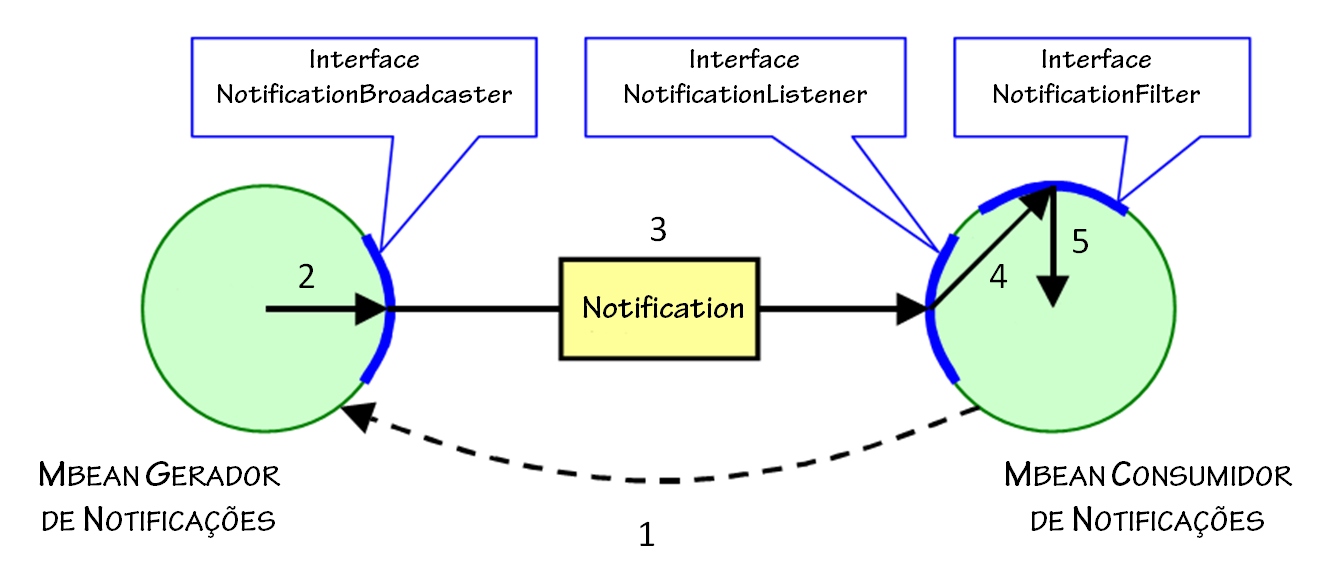
\includegraphics[width=13cm]{chapters/chapter2/notification_model.png}
\caption[Modelo de notificação JMX]{Modelo de notificação JMX~\cite{pericasgerencia}.}
\label{fig:notifyjmx}
\end{figure}

Na prática, JMX é uma tecnologia de monitoramento e notificação flexível, dinâmica e extensível, sendo utilizada em diversas ferramentas comerciais (\textit{e.g. } JBoss Application Server - JBoss~\cite{jboss}, JOnAS Application Server - OW2 Consortium~\cite{jonas}, Tivoli Composite Application Manager - IBM~\cite{tivoli}). 

\section{Ciclo PDCA}
\label{sec:pdca}
O ciclo PDCA (\textit{\textbf{P}lain \textbf{D}o \textbf{C}heck \textbf{A}ct}), ou ciclo de  Demming, é um ciclo de desenvolvimento e gestão de processos com foco na melhoria contínua ~\cite{shewhart}. O ciclo é dividido em 4 etapas, ver Figura \ref{fig:pdca}, que visam garantir o alcance de metas pré-estabelecidas, através da utilização de informações como fator chave na tomada de decisões.

O ciclo é aplicável a diversas atividades de gestão, incluindo o gerenciamento de performance~\cite{pdcacont}. Ele é um método eficaz de controle de atividades relacionadas à melhorias e compartilha dos conceitos de gerência de redes e recursos em geral, a medida que, a tomada de decisão é fortemente influenciada pelas informações coletadas.


\begin{figure}[htp]
\centering
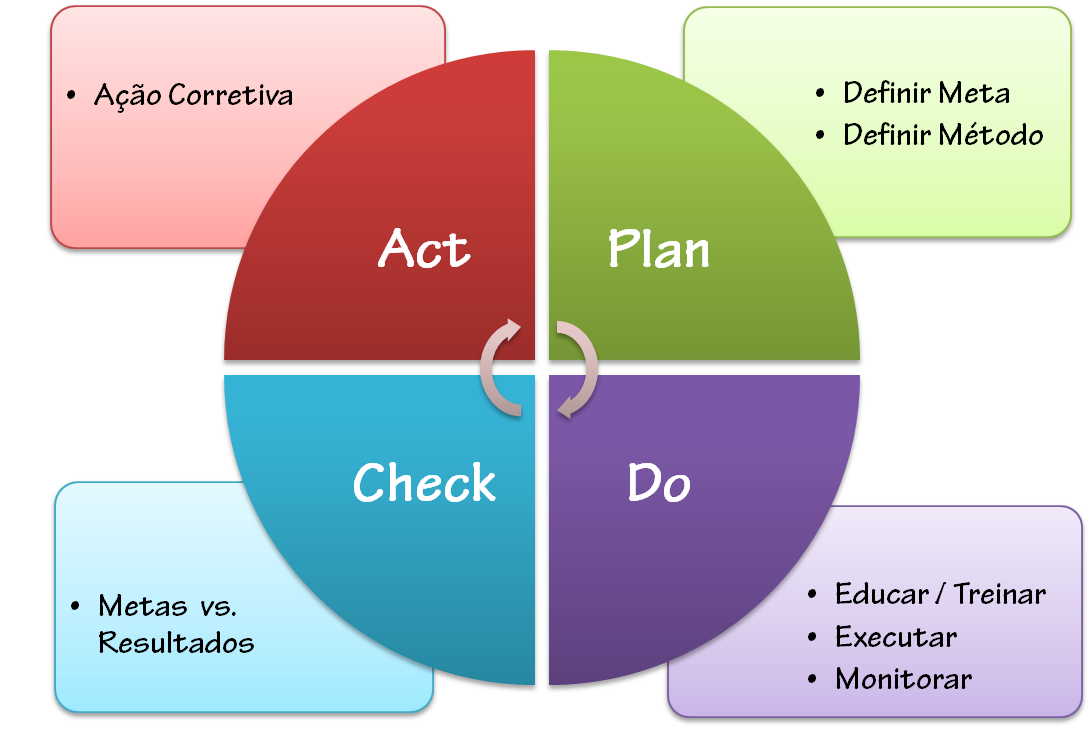
\includegraphics[width=7.5cm]{chapters/chapter2/pdca_cycle.png}
\caption[Ciclo PDCA]{Ciclo PDCA de Desenvolvimento com Foco na Melhoria Contínua.}
\label{fig:pdca}
\end{figure}


\subsection{Etapas}
\label{pdca:phases}
\subsubsection{\textit{Plan} - Planejar}
A fase de planejamento consiste no estabelecimento de metas e objetivos com base nas políticas adotadas pela organização~\cite{pdcacont}. Nesta etapa, é de extrema importância a análise de informações para a identificação e o entendimento do problema a ser resolvido. Esta é a fase mais importante do processo, uma vez que, um planejamento bem elaborado reflete no resultado como um todo. Evitando falhas e perda de tempo em fases futuras~\cite{fabio2003}~\cite{pdcacont}.

A fase de planejamento, resulta na elaboração de um plano de ação, que define os métodos necessários para atingir as metas estabelecidas.

\subsubsection{\textit{Do} - Executar}
É nesta fase em que ocorre a execução do plano de ação e coleta dos dados relacionados, para posterior análise~\cite{pdcacont}.

Nesta etapa é importante que a execução seja coerente com o plano de ação definido na fase anterior, uma vez que, enquanto a fase anterior busca maior eficácia e coesão, a fase de execução é voltada à eficiência do processo.

\subsubsection{\textit{Check} - Verificar}
Nesta etapa, é realizada a verificação dos resultados obtidos da execução realizada na fase anterior. Com base nas metas e estratégias definidas na fase de planejamento em conjunto com os dados monitorados na fase de execução, a etapa de verificação foca na análise sistemática dos dados monitorados a fim de verificar a efetividade das ações tomadas~\cite{pdcacont}. A diferença entre o desejável, o planejamento, e o resultado alcançado constitui um problema a ser resolvido.

\subsubsection{\textit{Act} - Agir}
Nesta fase são realizadas as ações corretivas, com base na análise do resultados da fase anterior. Essas ações tem o intuito de evitar que o problema verificado na etapa anterior volte a acontecer~\cite{pdcacont}. Essas ações também estão definidas no plano de ação e além de buscar corrigir problemas, podem estar envolvidas na busca por melhoria contínua do processo~\cite{pdcaknow}.

\paragraph{}
A aplicação dessas etapas resulta no aprendizado do processo, o que repercute na tomada de decisão, uma vez que, utiliza de informações relevantes extraídas da execução do processo.

\section{Considerações Finais}
Este capítulo apresentou os conceitos essenciais ao entendimento dos próximos capítulos e do trabalho como um todo. Apresentamos os paradigmas de orientação a serviços e componentes, assim como as plataforma OSGi e iPOJO, que são bases tecnológicas do mecanismo proposto. Por fim, demos uma visão geral do ciclo de desenvolvimento PDCA e da tecnologia de monitoramento de recursos utilizada neste trabalho, a tecnologia JMX.